\definecolor{caoplus}{HTML}{0072B2}
\definecolor{caominus}{HTML}{D55E00}
\begin{tikzpicture}[font=\scriptsize,
  ax/.style={-{Stealth[length=1.3mm]},line width=0.55pt},
  atm/.style={inner sep=0.3pt}]
\node[anchor=south west,inner sep=0] at (0,0) {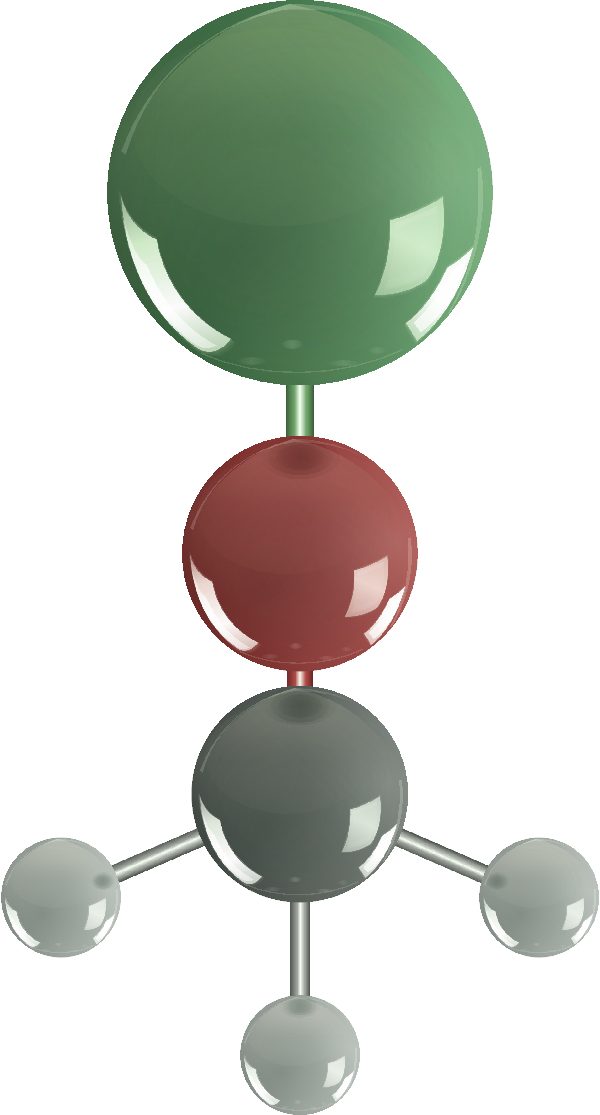
\includegraphics[width=2cm]{caoch3_molecule.pdf}};
\coordinate (o) at (1,2.35);
\draw[black!70,dashed,line width=0.4pt] (1,-0.15)--(1,4.25);
\draw[ax] (1,4.25)--(1,4.6) node[above=0.5pt] {$z$};
\draw[ax] (o)--(0.28,1.92) node[left=0.3pt] {$x$};
\draw[ax] (o)--(2.25,2.35) node[right=0.3pt] {$y$};
\draw[line width=0.45pt,black!45] ({1+0.86*cos(180)},3.05) arc[start angle=180,end angle=360,x radius=0.86cm,y radius=0.21cm];
\draw[line width=0.45pt,black!45] ({1+0.86},3.05) arc[start angle=0,end angle=42,x radius=0.86cm,y radius=0.21cm];
\draw[line width=0.45pt,black!45] ({1-0.86},3.05) arc[start angle=180,end angle=138,x radius=0.86cm,y radius=0.21cm];
\draw[-{Stealth[length=1.3mm]},line width=0.8pt,draw=caoplus]  ({1+0.86*cos(285)},{3.05+0.21*sin(285)}) arc[start angle=285,end angle=345,x radius=0.86cm,y radius=0.21cm];
\draw[-{Stealth[length=1.3mm]},line width=0.8pt,draw=caominus] ({1+0.86*cos(255)},{3.05+0.21*sin(255)}) arc[start angle=255,end angle=195,x radius=0.86cm,y radius=0.21cm];
\node[text=caoplus,anchor=west]  at (1.86,2.9) {$n_+$};
\node[text=caominus,anchor=east] at (0.14,2.9) {$n_-$};
\draw[black!60,densely dotted,line width=0.5pt] (0.05,4.12)--(1,4.12);
\draw[ax,line width=0.7pt] (o)--(0.05,4.12) node[above left=-1pt] {$\mathbf N$};
\draw[line width=0.5pt] (0.93,4.12)--(1.07,4.12) node[right=0.5pt] {$k$};
\node[atm,text=black] at (1.8,3.4) {Ca};
\node[atm,text=black] at (1.5,2) {O};
\node[atm,text=black] at (1.5,1.1) {C};
\node[atm] at (0.22,0.4) {H};
\draw[black!70,dashed,line width=0.4pt] (1.55,-0.15)--(1.55,0.55);
\draw[ax] (1.55,-0.15)--(2.08,0.38) node[above right=-1pt] {lab $Z$};
\draw[line width=0.4pt] (1.55,0.2) arc[start angle=90,end angle=45,radius=0.35cm];
\node at (1.72,0.38) {$\beta$};
\end{tikzpicture}
